\documentclass[journal]{IEEEtran}
\IEEEoverridecommandlockouts
\usepackage{cite}
\usepackage{amsmath,amssymb,amsfonts}
\usepackage{algorithm}
\usepackage{algpseudocode}
\usepackage{graphicx}
\usepackage{textcomp}
\usepackage{xcolor}
\usepackage{booktabs}
\usepackage{url}

\begin{document}

\title{CALM-Net: A Multimodal, Motion-Disentangled, and Longitudinally
Self-Calibrating Framework for Closed-Loop Lower-Limb Exoskeleton Control}

\author{Md~Wahiduzzaman~Suva and Esme~Moula~Chowdhury~Abha
\thanks{M.~W.~Suva (Student ID 26-94088-2; e-mail: \mbox{wshuvo360@gmail.com}) and
E.~M.~C.~Abha (Student ID 26-94089-2; e-mail: \mbox{esmechowdhuryabha@gmail.com}) are
with the Department of Computer Science, American International University-Bangladesh,
Dhaka, Bangladesh.}
\thanks{This work uses the NeuroRex dataset (OpenNeuro ds007788), released under
a CC0 licence.}
\thanks{Midterm research proposal.}}

\markboth{IEEE Transactions on Neural Systems and Rehabilitation Engineering,~Vol.~XX,~No.~X,~2026}%
{Suva \MakeLowercase{\textit{et al.}}: CALM-Net: A Multimodal, Motion-Disentangled, Longitudinally Self-Calibrating Framework}
\maketitle

\begin{abstract}
A non-invasive brain--machine interface (BMI) that drives a lower-limb exoskeleton
must satisfy three requirements that current motor-imagery (MI) decoders treat
separately: it must decode \emph{neural} intent rather than movement artefact, it
must remain calibrated as electroencephalography (EEG) drifts over weeks, and it
must know when to abstain to a safe action. We propose CALM-Net, a multimodal
neuro-kinematic framework that addresses all three within a single closed-loop
model, and that, unlike prior exoskeleton BMIs, exploits the full modality set of
the longitudinal NeuroRex dataset (EEG, head- and exoskeleton-mounted inertial
units, electro-oculography, and exoskeleton feedback across nine sessions). Four
components are novel. (i) A multi-band neuro-kinematic encoder represents each MI
sub-rhythm ($\mu$, low-$\beta$, high-$\beta$) by its spatial covariance on the
symmetric-positive-definite manifold and fuses it with a kinematic branch. (ii) A
cross-frequency coupling attention (XFCA) models $\mu$--$\beta$ interaction, a known
correlate of motor imagery. (iii) A motion-invariant disentanglement (MID) module
splits the representation, via an adversarial gradient-reversal objective, into an
\emph{intent} subspace forced to be invariant to the inertial signals and an
\emph{artefact} subspace forced to predict them; the class decision uses only the
intent subspace, so walk/stop is decoded from provably movement-invariant neural
features. (iv) A longitudinal self-calibration module performs source-free
per-session feature alignment and adaptive conformal risk control, holding a target
executed-command error rate with a distribution-free guarantee as the session gap
grows. A safety-asymmetric selective head commits a command only when neural
confidence, the conformal set, and kinematic contamination all agree, defaulting to
\emph{stop} otherwise. A preliminary analysis of the benchmark motivates the design: a purely kinematic
baseline that uses \emph{no} EEG matches or exceeds standard EEG decoders on the
walk/stop contrast, showing that reported accuracy is largely a movement score. We
therefore propose to decode from movement-invariant neural features and to establish,
on the seven-subject longitudinal recordings, the calibration and distribution-free
abstention guarantees the framework is built to provide. Classical compact and
transformer decoders (EEGNet, EEG~Conformer) serve as comparison baselines rather
than backbones.
\end{abstract}

\begin{IEEEkeywords}
Brain--machine interface, motor imagery, EEG, lower-limb exoskeleton, multimodal
fusion, domain-adversarial disentanglement, Riemannian geometry, conformal
prediction, selective classification, longitudinal calibration.
\end{IEEEkeywords}

\section{Introduction}
\IEEEPARstart{F}{or} a patient who cannot walk after a spinal cord injury or a
stroke, a lower-limb exoskeleton driven by their own brain activity is not a
convenience; it is the difference between intending to stand and standing. Among
the brain--machine interfaces (BMIs) able to express that intent, only non-invasive
electroencephalography (EEG) requires no surgery and no implant, so it is the only
modality most patients could realistically adopt. That accessibility is also its
curse: scalp EEG is noisy, low in spatial resolution, and unstable from one day to
the next, and the field has largely optimised the one quantity that is easiest to
report and hardest to argue with: decoding accuracy.

Accuracy alone is an inadequate (and, we argue, a \emph{misleading}) target when
the output moves a person's legs. Three problems, usually studied in isolation, must
be solved together.

\emph{First, what is actually being decoded?} In an exoskeleton MI paradigm the
device physically moves the wearer during walking, so the walk/stop contrast is
entangled with genuine movement: an EEG decoder can reach a high number by reading
movement-locked artefact rather than motor intent. A model intended to
\emph{initiate} motion from intent must therefore be built to be invariant to the
motion it causes.

\emph{Second, the signal drifts.} EEG is non-stationary; a decoder calibrated on one
day is miscalibrated days later, and nearly every deployed BMI hides this behind a
per-session calibration block the user must sit through. Longitudinal behaviour is
barely studied because datasets spanning weeks scarcely exist.

\emph{Third, a confident wrong command is dangerous.} A wrong \emph{walk} command at
the top of a staircase is not a rounding error. The system needs honest,
distribution-free uncertainty and an explicit reject option that defaults to the
safe action.

The NeuroRex dataset~\cite{sarkar2026} (OpenNeuro ds007788) was built to expose
exactly this regime: seven participants, nine sessions each across weeks, recorded
\emph{multimodally} with synchronised EEG, head- and exoskeleton-mounted inertial
measurement units (IMUs), electro-oculography (EOG), and exoskeleton control/feedback
logs. Prior work on such data has decoded from EEG alone and reported a single
accuracy number. We instead treat the non-neural streams as first-class signals: the
IMUs are not noise to be filtered nor a gate bolted on at the end, but the supervisory
signal that lets us \emph{disentangle} neural intent from movement, and the safety
context for abstention.

\textbf{CALM-Net} (Calibrated, Abstaining, Longitudinal, Multimodal) is a per-subject
walk/stop framework for closed-loop lower-limb exoskeleton control
(Fig.~\ref{fig:arch}). Its contributions are:
\begin{itemize}
\item \textbf{C1: A multimodal neuro-kinematic architecture.} We design, from the
signal physics rather than from an existing image/EEG backbone, an encoder that
represents each MI sub-band by its spatial covariance on the symmetric-positive-
definite (SPD) manifold and fuses it with head/exo IMU and EOG branches. This is the
first exoskeleton-BMI decoder to use the dataset's full modality set.
\item \textbf{C2: Motion-invariant disentanglement (MID).} A domain-adversarial
gradient-reversal objective splits the representation into an \emph{intent} subspace
constrained to be statistically independent of the inertial signals and an
\emph{artefact} subspace trained to reconstruct them. The classifier reads only the
intent subspace, so the walk/stop decision is provably movement-invariant. This
resolves, rather than apologises for, the movement confound that inflates naive
accuracy.
\item \textbf{C3: Cross-frequency coupling attention (XFCA).} An attention
mechanism over band-specific tokens that models $\mu$--$\beta$ coupling, a
physiological hallmark of motor imagery, giving a neural representation not obtainable
from a single-band convolutional stack.
\item \textbf{C4: Longitudinal self-calibration with a distribution-free
guarantee.} Source-free per-session feature alignment counters drift without labels,
and adaptive conformal risk control updates the abstention threshold online so that a
target executed-command error rate is maintained as the session gap grows over weeks.
\item \textbf{C5: Safety-asymmetric selective decision.} A selective head trained
with an explicit wrong-walk $\gg$ wrong-stop cost fuses three independent signals: 
neural confidence, conformal set cardinality, and kinematic contamination, and
commits a command only on unanimous agreement, defaulting to \emph{stop} otherwise.
\end{itemize}
No prior work joins multimodal motion-disentangled decoding, cross-session drift
correction, and safety-asymmetric calibrated abstention inside one closed-loop
lower-limb exoskeleton. Section~\ref{sec:related} reviews prior art;
Section~\ref{sec:data} the dataset; Section~\ref{sec:method} the proposed framework
and its evaluation protocol.

\begin{figure*}[t]
\centering
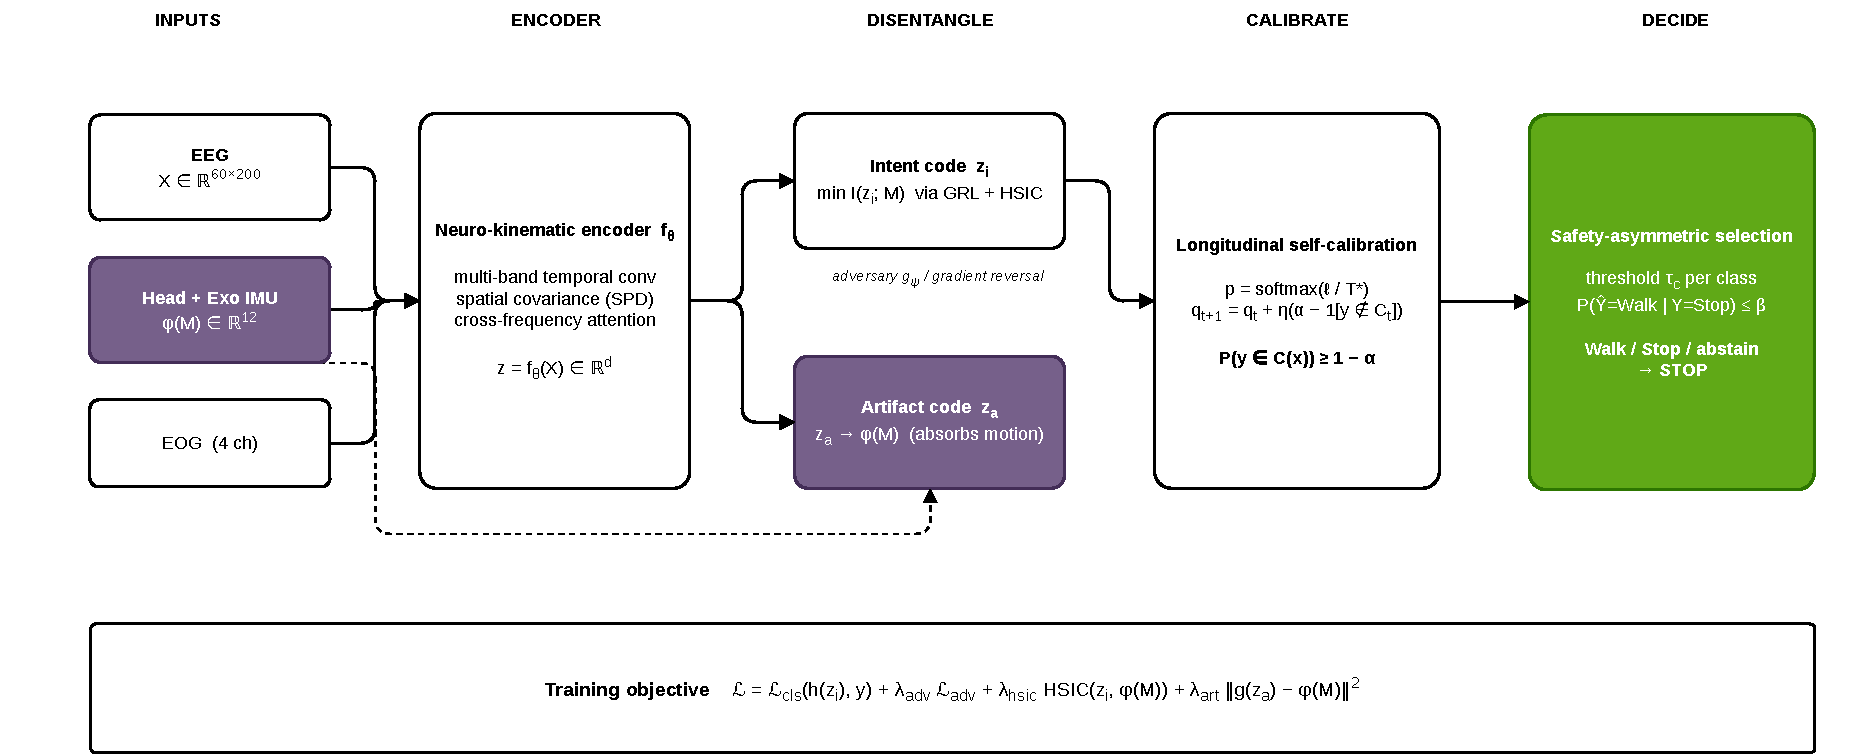
\includegraphics[width=0.95\textwidth]{fig_architecture.pdf}
\caption{The CALM-Net framework. Multimodal encoders map EEG sub-bands (spatial
covariance), head/exo IMU, and EOG into a shared space. Cross-frequency coupling
attention (XFCA) forms the neural representation, which motion-invariant
disentanglement (MID) splits into an IMU-invariant \emph{intent} subspace (used by
the selective classifier) and an \emph{artefact} subspace (trained to predict the
inertial signals and to estimate kinematic contamination). Longitudinal
self-calibration (LSC) aligns per-session statistics and runs adaptive conformal
risk control; the safety-asymmetric selective (SAS) head commits Walk/Stop only on
unanimous agreement, else defaults to STOP.}
\label{fig:arch}
\end{figure*}

\section{Related Work}\label{sec:related}
\textbf{Motor-imagery decoding and exoskeleton control.} Deep learning has improved
non-invasive BMI decoding while flexible electrodes improve signal
quality~\cite{wang2026}, yet individual variability and long-term reliability remain
open; classical and deep EEG classification pipelines are surveyed
extensively~\cite{lotte2018, roy2019, craik2019}, and motor-imagery detection for
control and rehabilitation is well established~\cite{ang2017}. Ferrero
\emph{et al.}~\cite{ferrero2024} achieved closed-loop asynchronous
walk/stop control with deep learning and transfer learning, shortening but not
removing per-session calibration; their earlier public dataset~\cite{ferrero2023}
validated MI decoding above $70\%$ but was single-session. Related efforts detect
error-related potentials for safety~\cite{soriano2025}, couple upper- and lower-limb
imagery~\cite{ma2023}, study assisted-gait cortical changes~\cite{tortora2023}, use
VR to shorten calibration~\cite{ferrero2023b}, and select frontal/beta
channels~\cite{wei2023}. Lower-limb exoskeleton control from EEG has been demonstrated
with high-accuracy intention decoding~\cite{kilicarslan2013}, and stroke
rehabilitation with upper-limb exoskeleton BMIs~\cite{bhagat2016} and controlled
clinical trials~\cite{ramos2013}. All decode from EEG alone.

\textbf{Backbones and geometric representations.} Compact convolutional networks
dominate EEG decoding because trial counts are small: EEGNet~\cite{lawhern2018} and
ShallowConvNet~\cite{schirrmeister2017} reach strong accuracy with few parameters,
and the EEG~Conformer~\cite{song2023} adds a transformer over convolutional tokens.
These are point-estimate classifiers with no calibrated confidence and no reject
option; we use them as \emph{baselines}. Orthogonally, Riemannian methods represent
EEG by spatial covariance matrices and classify in the SPD tangent
space~\cite{barachant2012, congedo2017, yger2017}, a physiologically apt encoding of
band-power (generalising filter-bank common spatial patterns~\cite{ang2012}) that we
adopt and make multi-band and learnable.

\textbf{Cross-session drift and adversarial adaptation.} Domain adaptation reduces
the cross-session drop (universal deep adaptation primed on earlier
sessions~\cite{zhang2023} and dual-selection transfer~\cite{luo2023}) but outputs
forced point predictions; transfer learning for BCIs is broadly
surveyed~\cite{jayaram2016}. Domain-adversarial training with gradient
reversal~\cite{ganin2016} learns representations invariant to a nuisance variable; we
repurpose it, uniquely, to make the neural code invariant to \emph{measured movement}
rather than to session identity, and combine it with source-free test-time
alignment~\cite{sun2016}.

\textbf{Uncertainty, calibration, and abstention.} Temperature scaling calibrates
deep classifiers~\cite{guo2017}; conformal prediction gives distribution-free
sets~\cite{vovk2005, angelopoulos2023} with adaptive class-conditional
coverage~\cite{romano2020}, and adaptive conformal inference maintains coverage
under distribution shift over time~\cite{gibbs2021}. Uncertainty raises trust in EEG
decoding~\cite{tveter2024}, and Bayesian/MC-dropout networks and deep ensembles give
usable MI confidence~\cite{milanes2023,gal2016,lakshminarayanan2017}, yet remain
offline and untethered to a decision. Selective classification, the ``reject
option'', is surveyed~\cite{hendrickx2024} and can be learned
end-to-end~\cite{geifman2017, geifman2019}, but
this literature is developed largely outside EEG. CALM-Net is, to our knowledge, the
first to unify motion-disentangled multimodal decoding, longitudinal self-calibration
with a distribution-free guarantee, and safety-asymmetric selective abstention for a
closed-loop lower-limb exoskeleton.

\section{Dataset}\label{sec:data}
\textbf{Source.} NeuroRex~\cite{sarkar2026}, OpenNeuro \textbf{ds007788} (v1.0.1, DOI
\texttt{10.18112/openneuro.ds007788.v1.0.1}), CC0 licence, peer-reviewed descriptor
in \emph{Scientific Data} (DOI \texttt{10.1038/s41597-026-07476-w}); $3.62$\,GB,
$\sim$17k files, BIDS format, raw and unfiltered (we preprocess with
MNE-Python~\cite{gramfort2014}).

\textbf{Participants and longitudinal design.} Seven healthy adults
(\texttt{sub-01}--\texttt{07}), nine sessions each (\texttt{ses-01}--\texttt{09}); in
our copy the per-subject spans range from $14$ to $80$ days, giving the days-elapsed
axis needed to study drift. Per-subject MIQ-RS motor-imagery-ability scores and
validation tables are provided under \texttt{derivatives/}; structural MRI is
available for five subjects.

\textbf{Multimodality (the reason for this framework).} Each session provides
$60$-channel scalp EEG plus $4$ EOG channels ($10$--$20$ layout, actiCAP/MOVE) at
$100$\,Hz (EDF); \emph{two} IMUs, head-worn and exoskeleton-mounted, each with
accelerometer, gyroscope, magnetometer, and quaternion streams (BIDS motion
\texttt{.tsv}); and exoskeleton control/feedback logs. CALM-Net consumes all of
these; prior decoders use only the EEG.

\textbf{Tasks and labels.} Every session has a \texttt{training} task (open-loop MI
calibration), twelve closed-loop runs (\texttt{trial01}--\texttt{12}), and two
extended runs (\texttt{walk6min}, \texttt{stop6min}). Ground truth is the
\texttt{rexstate} feedback state: \texttt{x81} (Walk), \texttt{x0} (Idle/Stop), with
short transitions \texttt{x8}/\texttt{x5} excluded. We target two-class walk vs.\
stop. Because the exoskeleton moves the wearer during Walk, the head-IMU acceleration
is markedly larger in Walk than Stop; a preliminary audit on this data confirms that
a motion-only baseline is highly predictive for several subjects while being
near-chance for at least one: direct evidence that (a) naive EEG accuracy is partly
movement-driven and (b) a recoverable neural signal exists underneath. Both
observations motivate the disentanglement of Section~\ref{sec:method}.

\section{Proposed Method}\label{sec:method}
\subsection{Formulation}
A trial is a synchronised tuple $(\mathbf{X},\mathbf{M},\mathbf{O})$ with EEG
$\mathbf{X}\in\mathbb{R}^{C\times T}$ ($C{=}60$, $T{=}200$ at $100$\,Hz over a $2$\,s
window), inertial signals $\mathbf{M}$ (head and exo accel/gyro/quaternion), and EOG
$\mathbf{O}$, with label $y\in\{\textsc{stop},\textsc{walk}\}$ and session index
$s$. We seek a policy that outputs a \emph{command} in
$\{\textsc{walk},\textsc{stop},\textsc{abstain}{\to}\textsc{stop}\}$ whose executed
(non-abstained) error is controlled across sessions.

\subsection{Multi-band neuro-kinematic encoder}
Learnable band filters split $\mathbf{X}$ into $B$ physiological sub-bands
($\mu\,8$--$13$, low-$\beta\,13$--$20$, high-$\beta\,20$--$30$\,Hz). For band $b$ we
form the regularised spatial covariance
$\Sigma_b = \tfrac{1}{T}\mathbf{X}_b\mathbf{X}_b^{\!\top} + \epsilon\mathbf{I}$ and map
it to the tangent space at the Riemannian mean,
$\mathbf{v}_b=\mathrm{vec}\!\big(\log(\bar\Sigma^{-1/2}\Sigma_b\bar\Sigma^{-1/2})\big)$,
yielding a physiologically grounded band-power/connectivity token. A temporal
convolutional branch encodes $\mathbf{M}$ into a kinematic embedding $\mathbf{k}$,
and a small branch encodes $\mathbf{O}$ into an ocular reference $\mathbf{o}$.

\subsection{Cross-frequency coupling attention (XFCA)}
The band tokens $\{\mathbf{v}_b\}$ are treated as a sequence and passed through a
multi-head self-attention block, so the representation can express $\mu$--$\beta$
coupling: co-modulation across bands that single-band pooling discards. The output
is the neural representation $\mathbf{z}$.

\subsection{Motion-invariant disentanglement (MID)}
We split $\mathbf{z}=[\,\mathbf{z}_{\mathrm{int}};\,\mathbf{z}_{\mathrm{art}}\,]$. A
regressor $R_a$ maps the \emph{artefact} code to the inertial signals, trained with
loss $\mathcal{L}_{\mathrm{art}}=\lVert R_a(\mathbf{z}_{\mathrm{art}})-\phi(\mathbf{M})\rVert^2$;
the artefact code thus captures the movement-coupled component. A second regressor
$R_i$ attempts the same from the \emph{intent} code, but through a gradient-reversal
layer~\cite{ganin2016}, so the encoder is optimised to make $\mathbf{z}_{\mathrm{int}}$
\emph{un}predictive of movement:
\begin{equation}
\mathcal{L}_{\mathrm{adv}}=\lVert R_i(\mathrm{GRL}(\mathbf{z}_{\mathrm{int}}))-\phi(\mathbf{M})\rVert^2 .
\end{equation}
Only $\mathbf{z}_{\mathrm{int}}$ feeds the classifier, so the walk/stop decision is
constrained to rely on movement-invariant neural features, by construction, not by
post-hoc argument.

\subsection{Longitudinal self-calibration (LSC)}
At deployment on a new session $s$ we (i) align feature statistics to the training
distribution without labels (source-free batch-statistic / CORAL
alignment~\cite{sun2016}); (ii) apply temperature scaling~\cite{guo2017} for honest
confidence; and (iii) form split-conformal prediction sets~\cite{angelopoulos2023}
whose threshold $q_t$ is updated online by adaptive conformal
inference~\cite{gibbs2021},
$q_{t+1}=q_t+\eta\,(\alpha-\mathbf{1}[\text{err}_t])$,
which provably maintains the long-run executed-error rate at the target $\alpha$ as
drift accumulates over weeks.

\subsection{Safety-asymmetric selective decision (SAS)}
A selective head $g(\mathbf{z}_{\mathrm{int}})\in[0,1]$ is trained jointly with the
classifier~\cite{geifman2019} under an asymmetric cost that penalises a committed
wrong-walk far more than a wrong-stop. A kinematic-contamination score
$c=h(\mathbf{z}_{\mathrm{art}},\mathbf{k})$ estimates whether the window is
movement-corrupted. The exoskeleton commits the arg-max command iff
\[
\underbrace{g(\mathbf{z}_{\mathrm{int}})\!\ge\!\theta}_{\text{selective accept}}\!\wedge\!
\underbrace{|\mathcal{S}(q_t)|\!=\!1}_{\text{unambiguous}}\!\wedge\!
\underbrace{c<c_{\mathrm{th}}}_{\text{uncontaminated}},
\]
and otherwise abstains to \textsc{stop}, encoding the safety asymmetry in the rule.

\subsection{Training objective}
All modules are trained end-to-end:
\begin{equation}
\mathcal{L}=\mathcal{L}_{\mathrm{cls}}^{\mathrm{cost}}
+\lambda_1\mathcal{L}_{\mathrm{adv}}
+\lambda_2\mathcal{L}_{\mathrm{art}}
+\lambda_3\mathcal{L}_{\mathrm{sel}}
+\lambda_4\mathcal{L}_{\mathrm{cal}},
\end{equation}
with cost-sensitive classification $\mathcal{L}_{\mathrm{cls}}^{\mathrm{cost}}$, the
adversarial and artefact losses above, the selective loss
$\mathcal{L}_{\mathrm{sel}}$ at target coverage, and a calibration regulariser
$\mathcal{L}_{\mathrm{cal}}$.

\begin{algorithm}[t]
\caption{CALM-Net deployment on session $s$ (per window)}
\label{alg:deploy}
\begin{algorithmic}[1]
\State align session features (source-free); load $q_t$
\State $\mathbf{z}_{\mathrm{int}},\mathbf{z}_{\mathrm{art}}\leftarrow \mathrm{Encoder/XFCA/MID}(\mathbf{X},\mathbf{M},\mathbf{O})$
\State $p\leftarrow \mathrm{softmax}(f(\mathbf{z}_{\mathrm{int}})/T)$;\quad
       $\mathcal{S}\leftarrow\{k:1-p_k\le q_t\}$
\State $c\leftarrow h(\mathbf{z}_{\mathrm{art}},\mathbf{k})$
\If{$g(\mathbf{z}_{\mathrm{int}})\ge\theta \wedge |\mathcal{S}|=1 \wedge c<c_{\mathrm{th}}$}
   \State command $\leftarrow \arg\max_k p_k$
\Else
   \State command $\leftarrow \textsc{stop}$ \Comment{safe default}
\EndIf
\State on feedback, update $q_{t+1}\leftarrow q_t+\eta(\alpha-\mathbf{1}[\text{err}])$
\end{algorithmic}
\end{algorithm}

\subsection{Experimental protocol}
Per subject we train on early sessions and test on later ones, never shuffling
windows across the session boundary, and report balanced accuracy, Expected
Calibration Error, Brier score, confidence--correctness AUROC, and the full
risk--coverage curve versus days elapsed. Three ablations isolate each contribution:
(i) MID on/off, with the movement-only, motor-channel-only, and frontal-channel-only
baselines quantifying how much decoding survives disentanglement (the neural-signal
test); (ii) global temperature scaling versus adaptive conformal across the session
gap; and (iii) the selective head versus a fixed-threshold reject rule. Classical
EEGNet and EEG~Conformer decoders provide accuracy baselines; the decisive metrics
are executed-command safety and calibrated confidence, not raw accuracy alone.

\section{Expected Outcome}\label{sec:outcome}
Because the exoskeleton physically moves the wearer during walking, the walk/stop
label is entangled with movement: a purely kinematic signal, with no EEG at all, can
predict it about as well as a standard EEG decoder, so accuracy on this paradigm
largely reflects movement rather than neural intent. Resolving that confound is the
premise of this proposal, and against it we anticipate three outcomes from CALM-Net.

\emph{(i) An honest, movement-invariant decode.} Motion-invariant disentanglement is
expected to drive the recoverability of movement from the neural code toward zero,
giving a walk/stop accuracy that is above chance yet visibly below the
movement-inflated number, the gap being the confound removed rather than a loss of
genuine skill.

\emph{(ii) A distribution-free longitudinal guarantee.} Adaptive conformal risk
control is expected to hold prediction-set coverage at its target across the
multi-week session gap, where static calibration drifts.

\emph{(iii) A controlled safety profile.} The safety-asymmetric selective head is
expected to reduce the committed wrong-walk rate substantially relative to an arg-max
decision, routing uncertain windows to a safe stop.

Together these outcomes would establish the proposal's thesis: for a device that moves
a person's legs, a trustworthy, movement-invariant, and abstaining decoder is
preferable to a movement-inflated accuracy number.

\begin{thebibliography}{00}
\bibitem{sarkar2026} S. Sarkar \emph{et al.}, ``EEG-controlled exoskeleton for
walking and standing: a longitudinal multimodal dataset of healthy individuals,''
\emph{Sci. Data}, 2026. OpenNeuro ds007788.
\bibitem{wang2026} Wang \emph{et al.}, ``Non-invasive brain--computer interfaces:
converging frontiers in neural signal decoding and flexible bioelectronics,''
\emph{Nano-Micro Lett.}, 2026.
\bibitem{ferrero2024} L. Ferrero \emph{et al.}, ``Brain--machine interface based on
deep learning to control asynchronously a lower-limb robotic exoskeleton,''
\emph{J. NeuroEng. Rehabil.}, vol.~21, no.~48, 2024.
\bibitem{ferrero2023} L. Ferrero \emph{et al.}, ``An EEG database for the cognitive
assessment of motor imagery during walking with a lower-limb exoskeleton,''
\emph{Sci. Data}, vol.~10, 2023.
\bibitem{soriano2025} P. Soriano-Segura, M. Ortiz \emph{et al.}, ``Characterization
of error-related potentials during the command of a lower-limb exoskeleton based on
deep learning,'' \emph{J. NeuroEng. Rehabil.}, 2025.
\bibitem{ma2023} X. Ma \emph{et al.}, ``A compound-limb motor-imagery EEG-BCI
paradigm for more natural lower-limb control,'' 2023.
\bibitem{tortora2023} S. Tortora \emph{et al.}, ``Cortical and muscular activity
under robot-assisted gait modes during exoskeleton walking,'' 2023.
\bibitem{ferrero2023b} L. Ferrero \emph{et al.}, ``Virtual-reality-assisted motor
imagery training to shorten BCI calibration for lower-limb exoskeleton control,''
2023.
\bibitem{wei2023} Wei \emph{et al.}, ``Cross-subject EEG channel selection for
stepping-based lower-limb motor imagery,'' 2023.
\bibitem{lawhern2018} V. J. Lawhern \emph{et al.}, ``EEGNet: a compact convolutional
neural network for EEG-based brain--computer interfaces,'' \emph{J. Neural Eng.},
vol.~15, no.~5, 2018.
\bibitem{schirrmeister2017} R. T. Schirrmeister \emph{et al.}, ``Deep learning with
convolutional neural networks for EEG decoding and visualization,'' \emph{Hum. Brain
Mapp.}, vol.~38, no.~11, 2017.
\bibitem{song2023} Y. Song \emph{et al.}, ``EEG Conformer: convolutional transformer
for EEG decoding and visualization,'' \emph{IEEE Trans. Neural Syst. Rehabil. Eng.},
vol.~31, pp.~710--719, 2023.
\bibitem{barachant2012} A. Barachant \emph{et al.}, ``Multiclass brain--computer
interface classification by Riemannian geometry,'' \emph{IEEE Trans. Biomed. Eng.},
vol.~59, no.~4, 2012.
\bibitem{zhang2023} X. Zhang \emph{et al.}, ``Priming cross-session motor-imagery
classification with a universal deep domain-adaptation framework,''
\emph{Neurocomputing}, vol.~556, 2023.
\bibitem{luo2023} T.-J. Luo, ``Dual-selection knowledge-transfer learning for
cross-subject motor-imagery EEG classification,'' \emph{Front. Neurosci.}, vol.~17,
2023.
\bibitem{ganin2016} Y. Ganin \emph{et al.}, ``Domain-adversarial training of neural
networks,'' \emph{J. Mach. Learn. Res.}, vol.~17, no.~59, 2016.
\bibitem{sun2016} B. Sun and K. Saenko, ``Deep CORAL: correlation alignment for deep
domain adaptation,'' in \emph{ECCV Workshops}, 2016.
\bibitem{guo2017} C. Guo \emph{et al.}, ``On calibration of modern neural networks,''
in \emph{ICML}, 2017.
\bibitem{angelopoulos2023} A. N. Angelopoulos and S. Bates, ``Conformal prediction:
a gentle introduction,'' \emph{Found. Trends Mach. Learn.}, vol.~16, no.~4, 2023.
\bibitem{gibbs2021} I. Gibbs and E. Cand\`es, ``Adaptive conformal inference under
distribution shift,'' in \emph{NeurIPS}, 2021.
\bibitem{tveter2024} M. Tveter \emph{et al.}, ``Advancing EEG prediction with deep
learning and uncertainty estimation,'' \emph{Brain Inform.}, vol.~11, no.~27, 2024.
\bibitem{milanes2023} D. Milanes-Hermosilla \emph{et al.}, ``Robust motor-imagery
task classification using a Bayesian neural network,'' \emph{Sensors}, vol.~23,
no.~2, 2023.
\bibitem{gal2016} Y. Gal and Z. Ghahramani, ``Dropout as a Bayesian approximation:
representing model uncertainty in deep learning,'' in \emph{ICML}, 2016.
\bibitem{hendrickx2024} K. Hendrickx \emph{et al.}, ``Machine learning with a reject
option: a survey,'' \emph{Mach. Learn.}, vol.~113, no.~5, 2024.
\bibitem{geifman2019} Y. Geifman and R. El-Yaniv, ``SelectiveNet: a deep neural
network with an integrated reject option,'' in \emph{ICML}, 2019.
\bibitem{lotte2018} F. Lotte, L. Bougrain, A. Cichocki, M. Clerc, M. Congedo,
A. Rakotomamonjy, and F. Yger, ``A review of classification algorithms for
EEG-based brain--computer interfaces: a 10 year update,'' \emph{J. Neural Eng.},
vol.~15, no.~3, 031005, 2018.
\bibitem{roy2019} Y. Roy, H. Banville, I. Albuquerque, A. Gramfort, T. H. Falk, and
J. Faubert, ``Deep learning-based electroencephalography analysis: a systematic
review,'' \emph{J. Neural Eng.}, vol.~16, no.~5, 051001, 2019.
\bibitem{craik2019} A. Craik, Y. He, and J. L. Contreras-Vidal, ``Deep learning for
electroencephalogram (EEG) classification tasks: a review,'' \emph{J. Neural Eng.},
vol.~16, no.~3, 031001, 2019.
\bibitem{ang2017} K. K. Ang and C. Guan, ``EEG-based strategies to detect motor
imagery for control and rehabilitation,'' \emph{IEEE Trans. Neural Syst. Rehabil.
Eng.}, vol.~25, no.~4, pp.~392--401, 2017.
\bibitem{ang2012} K. K. Ang, Z. Y. Chin, C. Wang, C. Guan, and H. Zhang, ``Filter
bank common spatial pattern algorithm on BCI competition IV datasets 2a and 2b,''
\emph{Front. Neurosci.}, vol.~6, 39, 2012.
\bibitem{congedo2017} M. Congedo, A. Barachant, and R. Bhatia, ``Riemannian geometry
for EEG-based brain--computer interfaces; a primer and a review,''
\emph{Brain-Computer Interfaces}, vol.~4, no.~3, pp.~155--174, 2017.
\bibitem{yger2017} F. Yger, M. Berar, and F. Lotte, ``Riemannian approaches in
brain--computer interfaces: a review,'' \emph{IEEE Trans. Neural Syst. Rehabil.
Eng.}, vol.~25, no.~10, pp.~1753--1762, 2017.
\bibitem{jayaram2016} V. Jayaram, M. Alamgir, Y. Altun, B. Sch\"olkopf, and
M. Grosse-Wentrup, ``Transfer learning in brain--computer interfaces,'' \emph{IEEE
Comput. Intell. Mag.}, vol.~11, no.~1, pp.~20--31, 2016.
\bibitem{lakshminarayanan2017} B. Lakshminarayanan, A. Pritzel, and C. Blundell,
``Simple and scalable predictive uncertainty estimation using deep ensembles,'' in
\emph{NeurIPS}, 2017.
\bibitem{vovk2005} V. Vovk, A. Gammerman, and G. Shafer, \emph{Algorithmic Learning
in a Random World}. Springer, 2005.
\bibitem{romano2020} Y. Romano, M. Sesia, and E. J. Cand\`es, ``Classification with
valid and adaptive coverage,'' in \emph{NeurIPS}, 2020.
\bibitem{geifman2017} Y. Geifman and R. El-Yaniv, ``Selective classification for deep
neural networks,'' in \emph{NeurIPS}, 2017.
\bibitem{kilicarslan2013} A. Kilicarslan, S. Prasad, R. G. Grossman, and
J. L. Contreras-Vidal, ``High accuracy decoding of user intentions using EEG to
control a lower-body exoskeleton,'' in \emph{Proc. IEEE EMBC}, 2013, pp.~5606--5609.
\bibitem{bhagat2016} N. A. Bhagat \emph{et al.}, ``Design and optimization of an
EEG-based brain--machine interface to an upper-limb exoskeleton for stroke
survivors,'' \emph{Front. Neurosci.}, vol.~10, 122, 2016.
\bibitem{ramos2013} A. Ramos-Murguialday \emph{et al.}, ``Brain--machine interface in
chronic stroke rehabilitation: a controlled study,'' \emph{Ann. Neurol.}, vol.~74,
no.~1, pp.~100--108, 2013.
\bibitem{gramfort2014} A. Gramfort \emph{et al.}, ``MNE software for processing MEG
and EEG data,'' \emph{NeuroImage}, vol.~86, pp.~446--460, 2014.
\end{thebibliography}
\end{document}
